61. $f(x)=x^2-|2x-2|-1=\begin{cases} x^2-2x+1,\ x\geqslant1,\\ x^2+2x-3,\ x<1.\end{cases}$
$$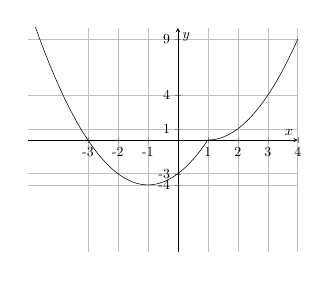
\begin{tikzpicture}[scale=0.5]
\begin{axis}[
    axis lines = middle,
    grid=major,
    legend pos={south west},
    xlabel = {$x$},
    %xlabel style={below right},
    ylabel = {$y$},
    ymin=-10,
    ymax=10,
    xmin=-5,
    xmax=4,
    xtick={-2,-3,-1,1,2,3,4,6},
    xticklabels={-2,-3,-1,1,2,3,4,6},
    ytick={-4,-3,1,4,9,25},
    yticklabels={-4,-3,1,4,9,25},
                  ]
	\addplot[domain=-5:4, samples=100, color=black] {x*x-abs(2*x-2)-1};
    %\addplot[domain=2.01:6, samples=100, color=black] {2/(2-x)};
   % \addplot[domain=-3:3, samples=100, color=black] {-x};
     %\addlegendentry{$\text{Рис. 1}$};
\end{axis}
%\draw (3.04,3.42) circle (2pt);
\end{tikzpicture}$$
По графику определим $E(f)=[-4;+\infty).$\\
